% Zużycie energii - może podłączyć pod rozdział 2.???
\section{Wstęp do badania zużycia energii}
\cite{noauthor_um1718_2022} jako podstawa dla części teoretycznej. Spróbować symulacji zużycia energii z użyciem PCC w Cube'ie.
Dodatkowo, oprzeć się na literaturze i artykulach naukowych, które poruszają tę kwestię - przynajmniej jeden.

Opisać tryby działania zarówno te przewidywane przez standard jak i te wprowadzone przez ST (niestety, jedyną dokumentacją jest kod).

\lipsum[1-10]

\section{Wstęp do badania Packet Error Rate}
<<do refaktoringu>>
\lipsum[1-3]

% poniższe sekcje przerzucić do części teoretycznej
\subsubsection{Definicja pakietu}
Przed przystąpieniem do badań należy precyzyjnie zdefiniować wykorzystywaną terminologię.

Pakietem nazywamy pojedynczą porcję danych przetwarzaną na poziomie warstwy sieciowej modelu ISO OSI \cite{sa_tcpip_nodate}.
Warstwa ta umożliwia routing, adresowanie logiczne oraz przetwarzanie i~dostarczanie pakietów.

\begin{figure}[!ht]
	\centering 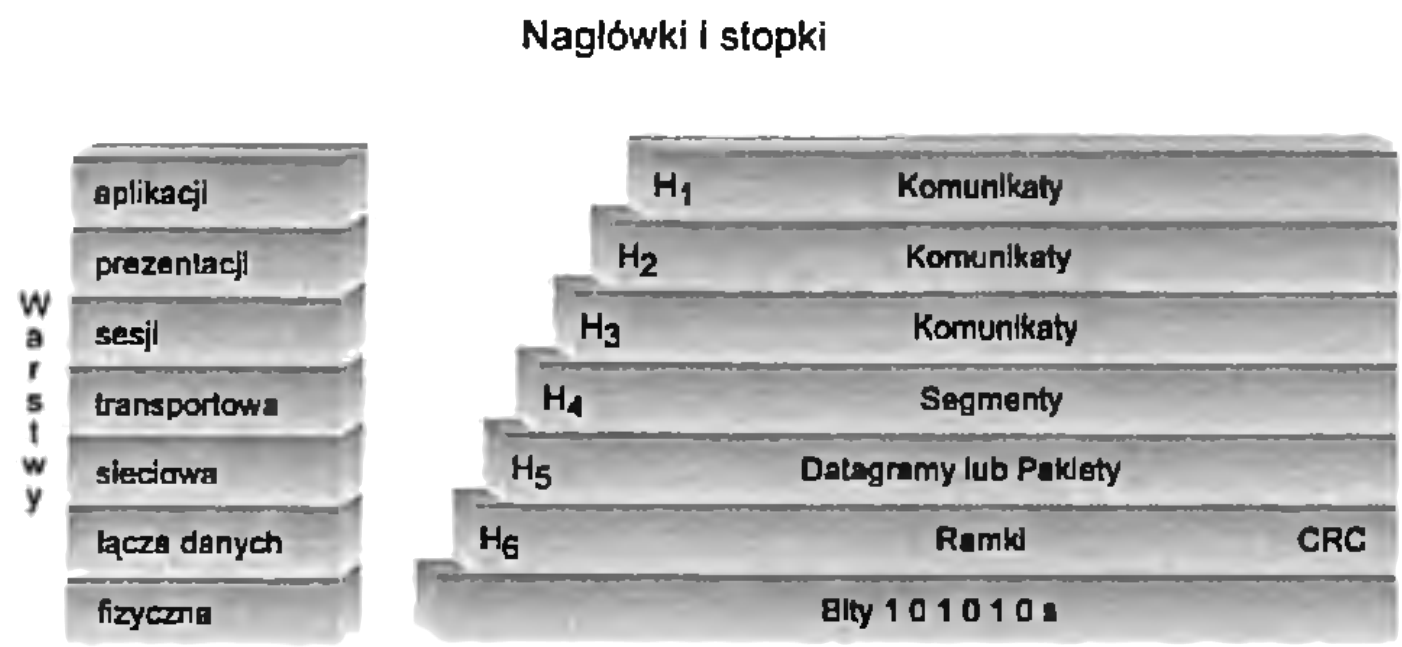
\includegraphics[width=0.618\linewidth]{tcp_ip_szkola_programowania_naglowki_stopki.png} 
	\caption{Model ISO OSI wraz i odpowiadające mu nazwy porcji danych. Źródło: \cite{sa_tcpip_nodate}}
	\label{rys:iso_osi_model_nazwy_grup_danych}
\end{figure}

\gls{BLE} wprowadza własną nomenklaturę dla poszczególnych warstw sieciowych. Jest to o tyle istotne, iż standard ten
nie zapewnia odpowiadających modelowi ISO OSI warstw jeden-do-jednego. Część z tych warstw jest agregowanych w~zespół 
protokołów wyższych warstw - Rysunek~\ref{rys:agregacja_protokolow_ble}. 

Bazując na definicji modelu OSI oraz stosie BLE, pakietem można nazwać wiadomości będące możliwie blisko
warstwy \textit{\gls{LL}}. Podobną definicję prezentuje dokumentacja ST:
\enquote{Pakiet to pojedyncza oznaczona wiadomość wysłana przez jedno i~odebrana przez 
co najmniej jedno urządzenie.}\footnote{Tłumaczenie własne}~\cite{stmicroelectronics_pm0271_2021}

\begin{figure}[!ht]
	\centering 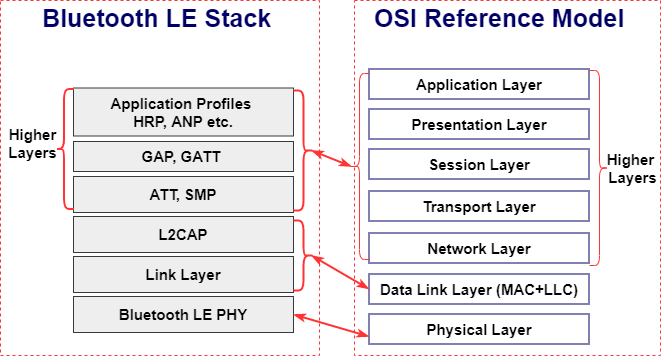
\includegraphics[width=0.618\linewidth]{mathworks_iso_osi_ble_stack.png} 
	\caption{Zestawienie stosu BLE i modelu ISO OSI. Źródło: \cite{noauthor_bluetooth_nodate}}
	\label{rys:agregacja_protokolow_ble}
\end{figure}

BLE Mesh dodatkowo wprowadza własne dodatkowe warstwy komunikacji, biorąc za podstawę stos BLE~\cite{mesh_working_group_mesh_2019}.
Każda z wymienionych warstw jest hermetyzowana za pośrednictwem dostarczanego przez producenta \gls{API}.
Uwzględniając zamknięcie middleware'u i dwu-procesorową architekturę mikrokontrolera STM32WB55, oznacza 
to brak możliwości bezpośredniego nasłuchiwania pakietów w~warstwie \gls{LL}.

Uwzględniając powyższe czynniki, \textit{pakietem} dla BLE Mesh nazywana będzie wiadomość najbliższa warstwie \gls{LL}.
W przypadku stworzonego oprogramowania, oznacza to odbiór komunikatu odebranego jako zdarzenie zarejestrowane przez
koprocesor Cortex-M0, będący integralną częścią mikrokontrolera STM32WB55 odpowiadający za obsługę radia.

\subsubsection{Definicja Packet Error Rate}
Posiadając definicję pakietu, \gls{PER} możliwe staje się zdefiniowanie wzoru, a~zarazem znaczenia
głównego celu badań.

PER jest miarą ilości błędnych pakietów w proporcji do wszystkich wysłanych pakietów, zgodnie ze wzorem:

\begin{equation}
\label{per_equation}
PER = \frac{s - r}{s} \cdot 100\%
\end{equation}

gdzie:

\begin{description}
\item[s] is ilość wysłanych pakietów
\item[r] is ilość odebranych pakietów
\item[s-r] - ilość niepoprawnych/błędnych pakietów
\end{description}

Powyższy wzór stanowi podstawę eksperymentu pozwalającego wyznaczyć jakość łącza w~zależności od
wybranych parametrów zmiennych.

\subsubsection{Wpływ tła radiowego na model}
* prezentacja hipotez
* przegląd literatury - jeśli jakaś istnieje...
* strefa Fresnela
* wpływ środowiska

